%% (Master) Thesis template
% Template version used: v1.4
%
% Largely adapted from Adrian Nievergelt's template for the ADPS
% (lecture notes) project.


%% We use the memoir class because it offers a many easy to use features.
\documentclass[11pt,a4paper,titlepage]{memoir}

%% Packages
%% ========

%% LaTeX Font encoding -- DO NOT CHANGE
\usepackage[OT1]{fontenc}

%% Babel provides support for languages.  'english' uses British
%% English hyphenation and text snippets like "Figure" and
%% "Theorem". Use the option 'ngerman' if your document is in German.
%% Use 'american' for American English.  Note that if you change this,
%% the next LaTeX run may show spurious errors.  Simply run it again.
%% If they persist, remove the .aux file and try again.
\usepackage[english]{babel}

%% Input encoding 'utf8'. In some cases you might need 'utf8x' for
%% extra symbols. Not all editors, especially on Windows, are UTF-8
%% capable, so you may want to use 'latin1' instead.
\usepackage[utf8]{inputenc}

%% This changes default fonts for both text and math mode to use Herman Zapfs
%% excellent Palatino font.  Do not change this.
\usepackage[sc]{mathpazo}

%% The AMS-LaTeX extensions for mathematical typesetting.  Do not
%% remove.
\usepackage{amsmath,amssymb,amsfonts,mathrsfs}

%% NTheorem is a reimplementation of the AMS Theorem package. This
%% will allow us to typeset theorems like examples, proofs and
%% similar.  Do not remove.
%% NOTE: Must be loaded AFTER amsmath, or the \qed placement will
%% break
\usepackage[amsmath,thmmarks]{ntheorem}

%% LaTeX' own graphics handling
\usepackage{graphicx}

%% We unfortunately need this for the Rules chapter.  Remove it
%% afterwards; or at least NEVER use its underlining features.
\usepackage{soul}

%% This allows you to add .pdf files. It is used to add the
%% declaration of originality.
\usepackage{pdfpages}

%% Some more packages that you may want to use.  Have a look at the
%% file, and consult the package docs for each.
%% See the TeXed file for more explanations

%% [OPT] Multi-rowed cells in tabulars
%\usepackage{multirow}

%% [REC] Intelligent cross reference package. This allows for nice
%% combined references that include the reference and a hint to where
%% to look for it.
\usepackage{varioref}

%% [OPT] Easily changeable quotes with \enquote{Text}
%\usepackage[german=swiss]{csquotes}

%% [REC] Format dates and time depending on locale
\usepackage{datetime}

%% [OPT] Provides a \cancel{} command to stroke through mathematics.
%\usepackage{cancel}

%% [NEED] This allows for additional typesetting tools in mathmode.
%% See its excellent documentation.
\usepackage{mathtools}

%% [ADV] Conditional commands
%\usepackage{ifthen}

%% [OPT] Manual large braces or other delimiters.
%\usepackage{bigdelim, bigstrut}

%% [REC] Alternate vector arrows. Use the command \vv{} to get scaled
%% vector arrows.
\usepackage[h]{esvect}

%% [NEED] Some extensions to tabulars and array environments.
\usepackage{array}

%% [OPT] Postscript support via pstricks graphics package. Very
%% diverse applications.
%\usepackage{pstricks,pst-all}

%% [?] This seems to allow us to define some additional counters.
%\usepackage{etex}

%% [ADV] XY-Pic to typeset some matrix-style graphics
%\usepackage[all]{xy}

%% [OPT] This is needed to generate an index at the end of the
%% document.
%\usepackage{makeidx}

%% [OPT] Fancy package for source code listings.  The template text
%% needs it for some LaTeX snippets; remove/adapt the \lstset when you
%% remove the template content.
\usepackage{listings}
\lstset{language=TeX,basicstyle={\normalfont\ttfamily}}

%% [REC] Fancy character protrusion.  Must be loaded after all fonts.
\usepackage[activate]{pdfcprot}

%% [REC] Nicer tables.  Read the excellent documentation.
\usepackage{booktabs}


%% Our layout configuration.  DO NOT CHANGE.
%% Memoir layout setup

%% NOTE: You are strongly advised not to change any of them unless you
%% know what you are doing.  These settings strongly interact in the
%% final look of the document.

% Dependencies
\usepackage{ETHlogo}

% Turn extra space before chapter headings off.
\setlength{\beforechapskip}{0pt}

\nonzeroparskip
\parindent=0pt
\defaultlists

% Chapter style redefinition
\makeatletter

\if@twoside
  \pagestyle{Ruled}
  \copypagestyle{chapter}{Ruled}
\else
  \pagestyle{ruled}
  \copypagestyle{chapter}{ruled}
\fi
\makeoddhead{chapter}{}{}{}
\makeevenhead{chapter}{}{}{}
\makeheadrule{chapter}{\textwidth}{0pt}
\copypagestyle{abstract}{empty}

\makechapterstyle{bianchimod}{%
  \chapterstyle{default}
  \renewcommand*{\chapnamefont}{\normalfont\Large\sffamily}
  \renewcommand*{\chapnumfont}{\normalfont\Large\sffamily}
  \renewcommand*{\printchaptername}{%
    \chapnamefont\centering\@chapapp}
  \renewcommand*{\printchapternum}{\chapnumfont {\thechapter}}
  \renewcommand*{\chaptitlefont}{\normalfont\huge\sffamily}
  \renewcommand*{\printchaptertitle}[1]{%
    \hrule\vskip\onelineskip \centering \chaptitlefont\textbf{\vphantom{gyM}##1}\par}
  \renewcommand*{\afterchaptertitle}{\vskip\onelineskip \hrule\vskip
    \afterchapskip}
  \renewcommand*{\printchapternonum}{%
    \vphantom{\chapnumfont {9}}\afterchapternum}}

% Use the newly defined style
\chapterstyle{bianchimod}

\setsecheadstyle{\Large\bfseries\sffamily}
\setsubsecheadstyle{\large\bfseries\sffamily}
\setsubsubsecheadstyle{\bfseries\sffamily}
\setparaheadstyle{\normalsize\bfseries\sffamily}
\setsubparaheadstyle{\normalsize\itshape\sffamily}
\setsubparaindent{0pt}

% Set captions to a more separated style for clearness
\captionnamefont{\sffamily\bfseries\footnotesize}
\captiontitlefont{\sffamily\footnotesize}
\setlength{\intextsep}{16pt}
\setlength{\belowcaptionskip}{1pt}

% Set section and TOC numbering depth to subsection
\setsecnumdepth{subsection}
\settocdepth{subsection}

%% Titlepage adjustments
\pretitle{\vspace{0pt plus 0.7fill}\begin{center}\HUGE\sffamily\bfseries}
\posttitle{\end{center}\par}
\preauthor{\par\begin{center}\let\and\\\Large\sffamily}
\postauthor{\end{center}}
\predate{\par\begin{center}\Large\sffamily}
\postdate{\end{center}}

\def\@advisors{}
\newcommand{\advisors}[1]{\def\@advisors{#1}}
\def\@department{}
\newcommand{\department}[1]{\def\@department{#1}}
\def\@thesistype{}
\newcommand{\thesistype}[1]{\def\@thesistype{#1}}

\renewcommand{\maketitlehooka}{\noindent\ETHlogo[2in]}

\renewcommand{\maketitlehookb}{\vspace{1in}%
  \par\begin{center}\Large\sffamily\@thesistype\end{center}}

\renewcommand{\maketitlehookd}{%
  \vfill\par
  \begin{flushright}
    \sffamily
    \@advisors\par
    \@department, ETH Z\"urich
  \end{flushright}
}

\checkandfixthelayout

\setlength{\droptitle}{-48pt}

\makeatother

% This defines how theorems should look. Best leave as is.
\theoremstyle{plain}
\setlength\theorempostskipamount{0pt}

%%% Local Variables:
%%% mode: latex
%%% TeX-master: "thesis"
%%% End:


%% Theorem environments.  You will have to adapt this for a German
%% thesis.
%% Theorem-like environments

%% This can be changed according to language. You can comment out the ones you
%% don't need.

\numberwithin{equation}{chapter}

%% German theorems
%\newtheorem{satz}{Satz}[chapter]
%\newtheorem{beispiel}[satz]{Beispiel}
%\newtheorem{bemerkung}[satz]{Bemerkung}
%\newtheorem{korrolar}[satz]{Korrolar}
%\newtheorem{definition}[satz]{Definition}
%\newtheorem{lemma}[satz]{Lemma}
%\newtheorem{proposition}[satz]{Proposition}

%% English variants
\newtheorem{theorem}{Theorem}[chapter]
\newtheorem{example}[theorem]{Example}
\newtheorem{remark}[theorem]{Remark}
\newtheorem{corollary}[theorem]{Corollary}
\newtheorem{definition}[theorem]{Definition}
\newtheorem{lemma}[theorem]{Lemma}
\newtheorem{proposition}[theorem]{Proposition}

%% Proof environment with a small square as a "qed" symbol
\theoremstyle{nonumberplain}
\theorembodyfont{\normalfont}
\theoremsymbol{\ensuremath{\square}}
\newtheorem{proof}{Proof}
%\newtheorem{beweis}{Beweis}


%% Helpful macros.
%% Custom commands
%% ===============

%% Special characters for number sets, e.g. real or complex numbers.
\newcommand{\C}{\mathbb{C}}
\newcommand{\K}{\mathbb{K}}
\newcommand{\N}{\mathbb{N}}
\newcommand{\Q}{\mathbb{Q}}
\newcommand{\R}{\mathbb{R}}
\newcommand{\Z}{\mathbb{Z}}
\newcommand{\X}{\mathbb{X}}

%% Fixed/scaling delimiter examples (see mathtools documentation)
\DeclarePairedDelimiter\abs{\lvert}{\rvert}
\DeclarePairedDelimiter\norm{\lVert}{\rVert}

%% Use the alternative epsilon per default and define the old one as \oldepsilon
\let\oldepsilon\epsilon
\renewcommand{\epsilon}{\ensuremath\varepsilon}

%% Also set the alternate phi as default.
\let\oldphi\phi
\renewcommand{\phi}{\ensuremath{\varphi}}


%% Make document internal hyperlinks wherever possible. (TOC, references)
%% This MUST be loaded after varioref, which is loaded in 'extrapackages'
%% above.  We just load it last to be safe.
\usepackage[linkcolor=black,colorlinks=true,citecolor=black,filecolor=black]{hyperref}


%% Document information
%% ====================

\title{Learned Single Shot Image-Based Camera Localization}
\author{Moyuan Zhou}
\thesistype{Master Thesis}
\advisors{Advisors: Dr. Bugra Tekin, Dr. Johannes L. Schönberger

Supervisor: Prof. Marc Pollefeys}
\department{Department of Computer Science}
\date{September 15, 2019}

\begin{document}

\frontmatter

%% Title page is autogenerated from document information above.  DO
%% NOT CHANGE.
\begin{titlingpage}
  \calccentering{\unitlength}
  \begin{adjustwidth*}{\unitlength-24pt}{-\unitlength-24pt}
    \maketitle
  \end{adjustwidth*}
\end{titlingpage}

%% The abstract of your thesis.  Edit the file as needed.
\begin{abstract}
  This example thesis briefly shows the main features of our thesis
  style, and how to use it for your purposes.
\end{abstract}

\clearpage
\renewcommand{\abstractname}{Acknowledgements}
\begin{abstract}
First and foremost, I would like to express my great gratitude to my advisors Dr. Bugra Tekin and Dr. Johannes L. Schönberger at Microsoft Research for their help this half year. They are very responsible and have provided countless advices to me during the whole period of my thesis. In this half year, we had weekly meetings regularly, and during each meeting they were responsive to the problems I was facing, gave me constructive suggestions and guided me to the potential directions with patience. The model we are using in this thesis also follows Bugra Tekin's work \cite{tekin2018real} last year.

I would like to show my special thanks to my supervisor Prof. Marc Pollefeys for offering the chance for me to work with Microsoft Research. I learnt quite a lot through this thesis  and gained both theoretical knowledge and practical experience in camera localization and object pose detection area.

I am also particularly grateful for the great help given by my friend Zuoyue Li. When I have some theoretical or implementing problems related with deep learning, Leonhard cluster, etc, he can always offer me quite valuable suggestions and help me solve the problem.

Last but not least, I would like to thank my  family especially my parents for their long-lasting spiritual and financial support throughout my studying life these years.

\end{abstract}
%% TOC with the proper setup, do not change.
\cleartorecto
\tableofcontents
\mainmatter

%% Your real content!
\chapter{Introduction}

In recent years, image-based camera localization has been a key task in the areas of augmented reality, virtual reality, robotics, autonomous driving, etc. There are many methods relying on RGB-D cameras which are quite robust and accurate. However, the RGB-D cameras are power consuming, which makes approaches based on mobile and wearable cameras more attractive. In this thesis, we focus on camera localization from RGB images and aim for real-time, efficient, and robust camera localization.

Traditionally, the PnP \cite{lepetit2009epnp} algorithm is used to solve the camera localization problem by computing the 6D camera pose given the 2D and 3D corresponding coordinates of multiple points. The fundamental problems of traditional approaches relying on local image features are textureless environments and robustness against strong changes in illumination/occlusion/viewpoint/etc. between the localized image and the given 3D model. To address these limitations, recently, deep learning has been applied to predict the 2D and 3D coordinates of these control points \cite{brachmann2017dsac} and has achieved superior results. However, these approaches are typically very time-consuming to train and evaluate. In this thesis, we want to combine the benefits of both worlds and develop a learned approach that is efficient and robust.

The problem of 6D object pose estimation from RGB images is related to the problem of camera localization. Recently, an efficient, single shot approach \cite{tekin2018real} for simultaneously detecting an object in an RGB image and predicting its 6D pose without requiring multiple stages has been proposed. This approach resulted in an improvement over the state-of-the-art in terms of accuracy and efficiency, and addressed the challenges on keypoint occlusion and multiple object pose estimation. In this project, we aim to adapt this approach for efficient image-based camera localization. To this end, we will define keypoints on the 3D room layout for indoor environments and predict the projections of these 3D keypoints. Camera pose with respect to the object will then be computed using PnP \cite{lepetit2009epnp} based on the correspondences between 2D predictions and 3D reference keypoints. Camera pose with respect to the scene can also be computed given the location of the 3D object in the scene.

The major challenges of the project include limited data for training the localization task, occlusion, and motion. We have generated labels for the ScanNet and SunCG dataset for this work which can also be used by future work in related area. To address occlusion and motion issues, one initial idea is to increase the number of keypoints without slowing down the method, which is a direction to go for higher accuracy and robustness. \cite{brachmann2017dsac} provided a trainable RANSAC approach for larger set of control points and can be integrated with the current model.


\section{Motivation}

In recent years, image-based camera localization has great and wide applications in multiple areas. Autonomous localization and navigation is necessary for a moving robot. Augment reality on images requires camera pose or localization. To view virtual environment, corresponding viewing angle needs to be computed.

Furthermore, unlike some other technics that require special devices, e.g. Lidar sensors, RGB-D cameras, etc, cameras are ubiquitous nowadays and people carry with their mobile phones that have cameras every day. Thus, we want to utilize only RGB images from 2D cameras to realize image-based camera localization.

As the current approaches are time-consuming \cite{brachmann2017dsac} or can not be generalized to new scenes \cite{wu2017delving}, we aim to come up with an efficient, real-time, and robust camera localization approach.


\section{Background}

\subsection{Overview on localization tools}

There are many localization tools nowadays, among which GPS is very commonly used outdoors, but it cannot be used indoors. Lidar, UWB, WiFi AP et al are effective indoor localization tools. However, they require special devices or data collections in advance. Compared to these tools, camera photos can provide higher discriminated features and more information, but in the same time require higher computation ability.

There are also many effective and robust methods relying on depth information acquired by RGB-D cameras currently. However, the RGB-D cameras are power consuming and not ubiquitous as 2D cameras. Thus, passive RGB images that are more commonly used and easy to be acquired by mobile devices and wearable cameras become more attractive. In this work we focus on RGB images that could be captured by 2D cameras, and do not rely on depth information. Compared to other localization tools, image-based camera localization is the most flexible and low cost one.

\subsection{Image-based camera localization}

Image-based camera localization \cite{wu2018image} is to compute camera poses under some world coordinate system from images or video captured by the cameras. Image-based camera localization can be classified into two categories according to that environments are prior or not: the one with known environments and the other one with unknown environments. Then one with known environments are usually the PnP problem studies, and the one with unknown environments consists of the methods with online and real-time environment mapping and the methods without online and real-time environment mapping. The former is commonly known as Simultaneous Localization and Mapping (SLAM) and the latter is the middle procedure of the commonly known structure from motion (SFM). In this thesis, we do not include any mapping or reconstruction procedure in our model since we are aiming for real-time localization given only single image as input, but for the training procedure 3D object model and object location in the scene is required as a prior knowledge.

There are also some approaches using convolutional neural network to predict camera pose directly from the 2D images or to compute 6D pose in some other way without using PnP algorithm. \cite{wu2017delving} predicts the orientation and translation of a camera given only a single picture. However, this approach is solving camera relocalization problem, and it can only predict in the same scene that the training period learnt. While this approach is useful in many robotic applications such as navigation and Simultaneous Localization and Mapping (SLAM), it cannot be generalised to a camera localization problem in a new/unseen scene. SSD-6D \cite{kehl2017ssd} relies on SSD architecture to predict 2D bounding boxes and a rough orientation estimate. Then based on the size of the 2D bounding box, it estimates the depth of the object and lift the 2D detection to 6D. However, the refinement step of this approach increases the running time a lot that cannot make a real-time prediction feasible.

Recently, a real-time single shot 6D object pose estimation approach \cite{tekin2018real} has been proposed. 6D object pose estimation is related with camera pose estimation which let us see a possibility of realizing real-time camera localization task in a general scene. \cite{tekin2018real} is using a single shot deep convolutional neural network to predict the 2D projections of the object's 3D bounding boxes, and then use a PnP algorithm to compute 6D object pose given the corresponding 2D coordinates and locations of 3D points. We adapt this approach for our camera localization task. Specifically, we use a PnP algorithm to calculate camera pose with respect to the object from the 2D coordinates predicted by the network and the corresponding 3D keypoints of some known 3D models. Usually, the ground truth of the %camera pose is given as the camera pose with respect to the scene. To make the result comparable with the ground truth, we need to compute camera location with respect to the scene applying the location of the object in the scene.

\subsection{PnP algorithm}

As we are applying PnP algorithm to calculate the camera pose according to some corresponding 2D and 3D points. Here is a introduction to PnP algorithm.

Camera pose determinations from known 3D space points are called perspective-n-point problem, namely PnP problem. Let n be the number of used points. When $n \geq 6$, the problem is linear. When $n = 3,4,5$, the problem is nonlinear. And when $n < 3$, there is no solution. Although the P3P problem has been well solved, but there may exist multiple solutions. In this work, we set the number of keypoints per object as 9. Although there may sometimes be outliers due to occlusion or other reasons, we can still guarantee it is a linear problem at most of the cases.

When the PnP problem is linear, there are also a lot of works studying on efficient optimizations for the camera poses from small number of points. \cite{lepetit2009epnp} provide an accurate O(n) solution to the PnP problem, called EPnP which is widely used today. In our approach, we also utilize EPnP and compare it with other PnP solutions.

\subsection{6D object pose estimation}

There are also lots of current works on 6D object pose estimation. Traditional approaches are mainly local image features extraction and matching. There are many fast keypoint and edge-based methods for textured objects, but not effective to weakly textured or untextured objects, or low resolution video streams.

Recently, deep learning methods are utilized in solving 6D object pose estimation problem and have achieved outstanding performance. BB8 \cite{rad2017bb8} is a 6D object detection pipeline made of one CNN to coarsely segment the object and another to predict the 2D locations of the projections of the object's 3D bounding box given the segmentation. It then use PnP algorithm to compute 6D pose using the corresponding points. The method is effective but slow due to its multi-stage nature. SSD-6D \cite{kehl2017ssd} is another approach which relies on SSD architecture to predict 2D bounding boxes and a very rough estimate of the object's orientation in a single step. Then the object's depth is approximated from the size of the 2D bounding box in the image and the 2D detection is lifted to 6D. However, both BB8 and SSD-6D methods require a post-processing step to refine the result, which increase the running time linearly and make the methods not feasible for real-time tasks.

\subsection{Constraints on image-based camera localization problem}

The common problem for camera localization or object pose detection is that the datasets available are rather limited, compared to datasets for other tasks like classification or tagging. Specifically, the most common datasets for detection contain thousands to hundreds of thousands of images with dozens to hundreds of tags, while classification datasets have millions of images with tens or hundreds of thousands of categories. Labeling images for detection is far more expensive than labeling for classification or tagging where tags are often user-supplied for free. These result in object detection problem lack of enough datasets and labels.

In this work, we generate the 2D projections of object's 3D bounding boxes for multiple objects as labels for indoor environments. We take ScanNet dataset as the realistic dataset and SunCG together with six tools for synthetic dataset. The labels generated can also be used in future works on related topics.


\section{Focus of this work}

As clarified in the previous background section, we are aiming for a real-time and robust image-based camera localization approach that can predict the camera pose in a new scene. The new scene could be in similar environment as the training scenes, e.g. indoor environment with furnitures, but they should not be the same scenes. The approach should also be able to generalise to various object with no need of precise and detailed texture.

We adapt the recent real-time single shot 6D object pose prediction approach \cite{tekin2018real} to our camera localization approach. We also generate new labels for indoor environment dataset. Basically, the approach uses a single shot deep CNN architecture to find the corresponding 2D image coordinates of the 3D ground keypoints for some known 3D models in the environments and then applies a PnP algorithm to calculate the camera pose with respect to the object. We choose the 3D keypoints as the 8 corners of the object's 3D bounding box plus the center point of the object. The network is single shot and end-to-end trainable, and the model is also accurate without requiring any post-processing, so it is faster than the other current existing methods which are multi-stage or require post-processing for pose refinement.
\chapter{Related Work}

In this chapter we review the existing works on camera localization from classical feature and template matching methods to newer end-to-end trainable CNN-based methods. Since we use 6D object pose estimation to realize our camera localization, object detection and 6D pose estimation related works are also reviewed.

\section{Camera localization methods}

\subsection{Classical methods}

Traditional camera pose estimation works \cite{irschara2009structure, lim2015real, lynen2015get, zeisl2015camera, sattler2016efficient} are mainly using local feature extraction and mapping. Most common approach to image-based localization is structure-based and tackles the problem by first matching the local 2D features of an image to the 3D point cloud model of the scene. Local descriptors needed by such methods were designed for invariance to changes in scale, rotation, illumination and viewpoints. Recent improvements has made these methods quite robust and accurate.

Recently, a privacy preserving image-based localization method \cite{speciale2019privacy} is proposed by lifting the map representation from a 3D point cloud to a 3D line cloud, which obfuscates the underlying scene geometry while providing sufficient geometric constraints to enable robust and accurate 6D camera pose estimation.

\subsection{CNN-based methods}
There are some CNN-based end-to-end camera pose prediction methods. \cite{wu2017delving} predicts the orientation and translation of a camera given only a single picture. However, this approach is solving camera relocalization problem, and it can only predict in the same scene that the training period learnt. While this approach is useful in many robotic applications such as navigation and Simultaneous Localization and Mapping (SLAM), it cannot be generalised to a camera localization problem in a new/unseen scene. 

In a recent image-based localization work using LSTMs for structured feature correlation \cite{walch2017image}, the authors propose a new CNN plus LSTM architecture for camera pose regression for indoor and outdoor scenes. In this approach, they use CNN to learn feature representations for localization, and use LSTM units to reduce structured dimensionality on the feature vector of the CNN output.

\section{Object detection based methods}
Camera location can also be computed from 6D object pose. 6D object pose detection approaches are mostly based on object detection means. Here we review related works from the initial R-CNN based object detection methods to the latest single shot 6D object pose detection method.

\subsection{Object detection}

\paragraph{YOLO}
YOLO is a real-time single shot object detection approach and is proposed in the same time as SSD. Most of the works for object detection before YOLO have a first step to propose possible regions of the object, and then do the classification and refinement. The multiple stages make the model hard to optimize since each component must be trained separately. The post-processing step also makes the training and prediction rather slow.

YOLO  frame object detection as a regression problem instead of the previous classification problem. Instead of doing classification on a proposed region, YOLO can predict the location of the bounding boxes of the object directly. Given a full image, YOLO use a single network to predict all bounding boxes across all classes for the image simultaneously in one evaluation. Thus, YOLO realizes a single shot, end-to-end trainable network for object detection task.

Although YOLO cannot achieve the state-of-the-art accuracy but it is extremely fast and capable for real-time object detection. Compared with other real-time systems, it has more than twice of the mean precision. Although YOLO has lower recall compared to region proposal-based methods, it has less than half false positives on background errors compared to Fast R-CNN.

There are some constraints of YOLO as well. The first one is that there is a limit on the number of nearby objects that the model can predict. Since YOLO partition the image into multiple grid, and each grid cell can only predict one class, although it can predict B bounding boxes per grid, there is still only one object predicted as output. If two objects are very close and have their center in the same grid, only one of them can be predicted. The second one is that YOLO does not achieve the state-of-art accuracy. There is significant number of localization errors and relatively low recall of YOLO compared to region proposal-based methods.

\paragraph{YOLO v2}
YOLO v2 has done some improvements to the YOLO detection method. Inspired by Faster R-CNN, which use the region proposal network(RPN) to predict offsets and confidences for anchor boxes, YOLO v2 removed the fully connected layer at the end of the network, and instead use anchor boxes to predict bounding boxes. YOLO v2 decouples the class prediction mechanism from the spatial location and instead predict class for every anchor box. In this way, the limitation of only one class is predicted per grid cell is released, and now we can better predict nearby objects.

YOLO v2 achieves a good tradeoff between speed and accuracy. It outperforms Faster R-CNN with ResNet and SSD while still running significantly faster. In this work, our network architecture is also based on YOLO v2.


\subsection{6D object pose detection}

\paragraph{BB8}
BB8 \cite{rad2017bb8} is a 6D object detection approach which consists of one CNN to realize a coarse segmentation and another to predict the 2D locations of the projections of the object’s 3D bounding box, which are then used by a PnP algorithm to compute the 6D object pose. The segmentation stage generates a 2D segmentation mask for presenting a cropped image to the second network. There is also an optional additional step that refines the predicted poses. The method is slow due to its multi-stage nature.

\paragraph{SSD-6D}
The SSD-6D \cite{kehl2017ssd} approach relies on the SSD architecture to predict object's 2D bounding boxes and a pool of the most likely 6D poses for that instance. It then predicts the approximated depth of the object from the size of the 2D bounding box in the image and lift the output from 2D to 6D object pose. In the final step, the approach refine each pose in every pool and select the best after verification. As the method require a refinement step to get a good accuracy, the running time is increased linearly with the number of objects being detected.

\paragraph{Real-time single shot approach}

The recently proposed real-time seamless single shot approach \cite{tekin2018real} performs 6D object pose prediction in an RGB image without multiple stages or hypotheses. It proposed a new CNN architecture which is inspired by YOLO and YOLO v2. The end-to-end trainable architecture makes it easy and fast to optimize. The approach turns out to be fast enough for real-time 6D object pose detection and accurate without requiring any additional post-processing.

The network is based on the YOLO v2 network but extends 2D detection to 6D detection task. It directly predicts the 2D image locations of the projected vertices of the object’s 3D bounding box and then use a PnP algorithm to predict the object’s 6D pose.

Compared with other approaches, the single shot approach outperforms BB8 \cite{rad2017bb8} and SSD-6D \cite{kehl2017ssd} when they are tested without post-processing - as we introduced above, BB8 and SSD-6D have pose refinement step as post-processing to boost the accuracy but with a cost of much slower performance. When handling multiple objects, the single shot approach virtually has no time-penalty, that is the running time remains constant, whereas other methods grow proportional to the number of objects.
\chapter{Example Chapter}

Dummy text.

\section{Example Section}

Dummy text.

\subsection{Example Subsection}

Dummy text.

\subsubsection{Example Subsubsection}

Dummy text.

\paragraph{Example Paragraph}

Dummy text.

\subparagraph{Example Subparagraph}

Dummy text.

\chapter{Datasets}

Dummy text.

\section{Dataset types}

Dummy text.

\subsection{Synthetic data}

Dummy text.
\subsubsection{Sixd}


\subsubsection{Suncg}


\subsection{Real data}
We aim to have a nice generalization of our model to real data. Thus, we mainly focus on the prediction result of our model on datasets consisting real data. In this subsection, we introduce some current datasets containing real data of indoor environments, and elaborate whether they are capable to be used in our work.

\subsubsection{NYU-Depth}
The NYU-Depth V2 dataset is comprised of video sequences from a variety of indoor scenes as recorded by both the RGB and Depth cameras from the Microsoft Kinect. It features 1449 densely labeled pairs of aligned RGB and depth images among 464 scenes taken from 3 cities plus 407,024 unlabeled frames. Each object in the data is labeled with a class and an instance number.

However, the dataset does not provide camera pose information or camera extrinsic parameters for each image, so there is no ground truth for camera location. It also doesn't provide any reconstructed 3D scenes or models, so that we cannot generate ground truth of the 2D coordinates labels for the corresponding 3D keypoints. Thus, NYU-Depth dataset is not applicable for our training or testing procedure.

\subsubsection{7-Scenes}
The 7-Scenes dataset is a collection of tracked RGB-D camera frames recorded from a handheld Kinect at $640 \times 480$ resolution. It uses KinectFusion system to obtain the ground truth camera tracks and a dense 3D model. Many works and applications in relocalization and dense tracking and mapping use 7-scenes for evaluation, such as the camera relocalization work from Wu et al \cite{wu2017delving}. While 7-Scenes are available for end-to-end camera pose learning methods, it does not suit for our object pose detection based method.

For the training procedure and labeling, our method needs the object's 3D model and position with respect to the camera as a prior knowledge. 7-Scenes has provided the dense reconstruction represented by signed distance volume of each scene. However, there is no category or object instance labeling related with the 3D scenes. Thus, we cannot get the 3D model and corresponding 2D labels for each object and train for 6D object pose detection. Also, there are limited number of scenes, 7 exactly, which is not enough for our training procedure, where we aim to generalize to as many as possible different scenes. 

During testing, we do not need the 3D object model any more for 6D object pose detection as long as there is trained category object exists in the image. However, our estimation of camera location is with respect to the object. If we have knowledge of the object 3D position with respect to the scene, we can also calculate the camera pose with respect to the scene. 7-Scenes only provides ground truth camera pose with respect to the scene, but do not have any knowledge of the object position. Thus, we cannot compute the camera location with respect to the scenes and 7-Scenes dataset is not applicable for evaluation in our method.

\subsubsection{Scannet}


\subsection{Dataset processing}

\paragraph{Ordre of corners}
\paragraph{Data filtering}


\chapter{Experiments and Results}

In this chapter, we present experiments we did in this work and some valuable results we have achieved. We did experiments in both synthetic data and real data. We started with synthetic data to check how well our model can predict camera location in synthetic data on exactly same objects. It turns out the network can predict quite accurately for synthetic data. Then we did experiments in real data. We hope that by mixing synthetic data together with real data as training data, we can improve the result of prediction in real data.

\section{Synthetic Data}

We first did experiments on multiple views of a single object generated by SIXD Toolkit. We use objects from SunCG, and we generate multiple views of the object in random texture, with random translation within the camera's field of view, and with random distance to the object. We are also training with data in random background, testing in both no background and random background. As a result, the prediction is very accurate. Taking a 5 px threshold, the accuracy that the error of 2D projection of all vertices of the object 3D mesh between prediction and ground truth within the threshold is greater than 70\%. Figure \ref{fig:sixd} shows the predictions on the test data of our generated synthetic data with no background. The red bounding box is the ground truth, the yellow box is the predicted 2D locations of the projected bounding box, the blue box is the reprojected bounding box using the camera pose computed from ground truth 2D locations i.e. the red box corners and given 3D control points locations, and finally the green box is the reprojected box using the camera pose computed from predicted 2D locations i.e. the yellow box corners and given 3D control points locations.

\begin{figure}[h!]
  \centering
  \begin{subfigure}[b]{0.32\linewidth}
    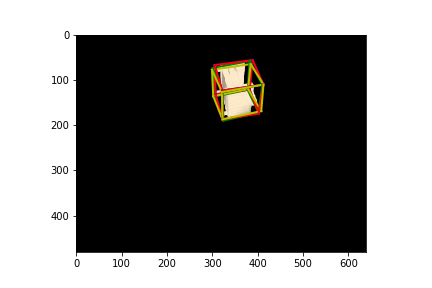
\includegraphics[width=\linewidth]{results/sixd/0267.png}
  \end{subfigure}
  \begin{subfigure}[b]{0.32\linewidth}
    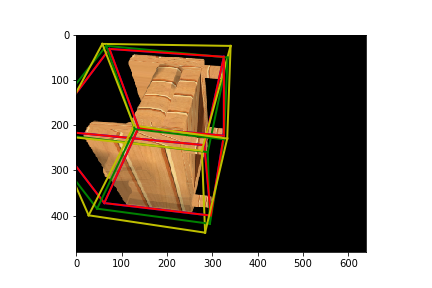
\includegraphics[width=\linewidth]{results/sixd/0298.png}
  \end{subfigure}
  \begin{subfigure}[b]{0.32\linewidth}
    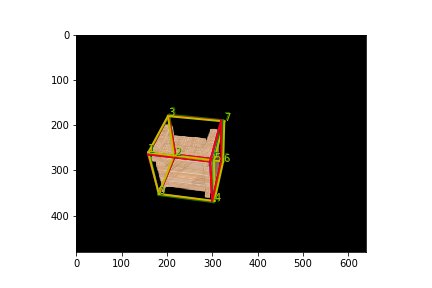
\includegraphics[width=\linewidth]{results/sixd/0501.png}
  \end{subfigure}
  \begin{subfigure}[b]{0.32\linewidth}
    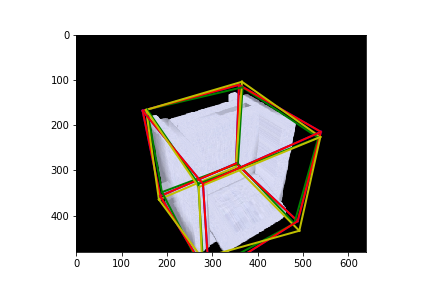
\includegraphics[width=\linewidth]{results/sixd/0529.png}
  \end{subfigure}
  \begin{subfigure}[b]{0.32\linewidth}
    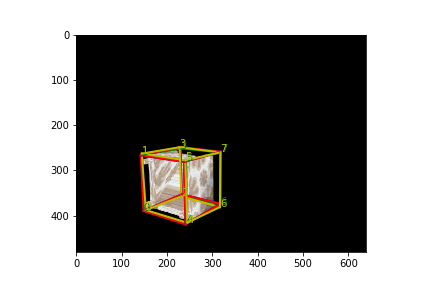
\includegraphics[width=\linewidth]{results/sixd/1151.png}
  \end{subfigure}
  \begin{subfigure}[b]{0.32\linewidth}
    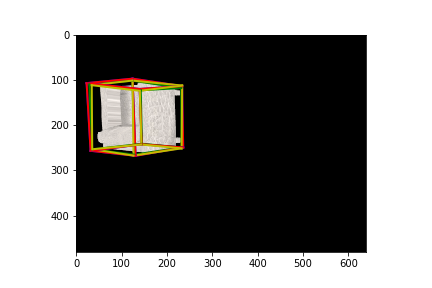
\includegraphics[width=\linewidth]{results/sixd/1186.png}
  \end{subfigure}
  \caption{Examples of results of sofa object in multiple views generated with SIXD Tookit}
  \label{fig:sixd}
\end{figure}

Then we did experiments on the whole synthetic image. We use SunCG toolbox to render the whole synthetic indoor environment images provided in SunCG dataset. Specifically, we filter out scenes containing our target object - sofa, render images of the scenes, and filter out images containing the object with the rules we stated in section \ref{sec:data_filtering}. Figure \ref{fig:suncg} shows the results of testing on SunCG dataset.

\begin{figure}[h!]
  \centering
  \begin{subfigure}[b]{0.32\linewidth}
    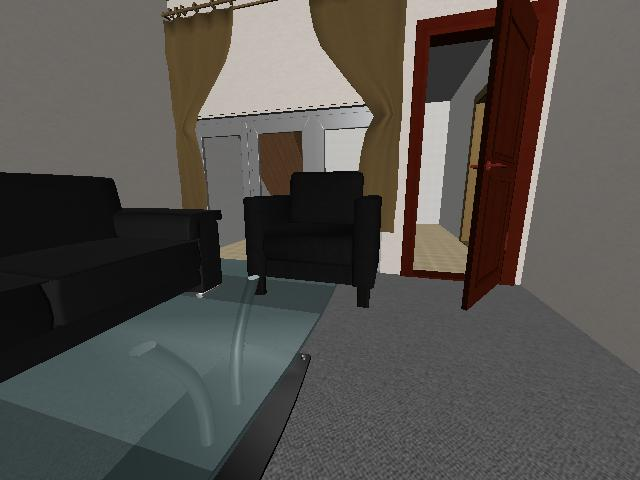
\includegraphics[width=\linewidth]{results/suncg/000004_color.jpg}
  \end{subfigure}
  \begin{subfigure}[b]{0.32\linewidth}
    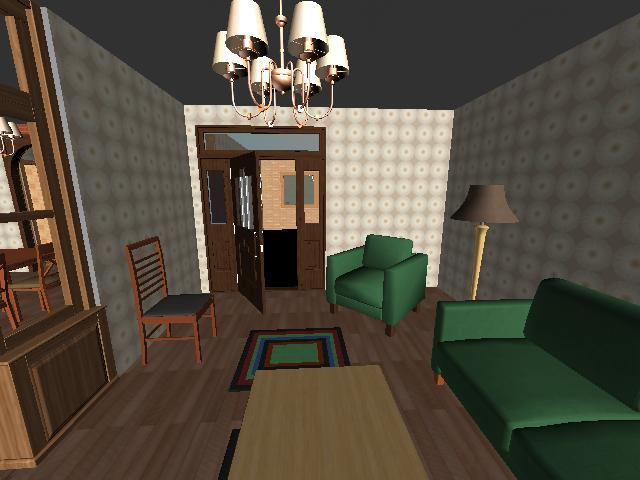
\includegraphics[width=\linewidth]{results/suncg/000005_color.jpg}
  \end{subfigure}
  \begin{subfigure}[b]{0.32\linewidth}
    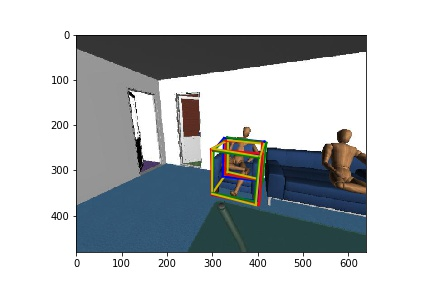
\includegraphics[width=\linewidth]{results/suncg/000006_color.jpg}
  \end{subfigure}
  \begin{subfigure}[b]{0.32\linewidth}
    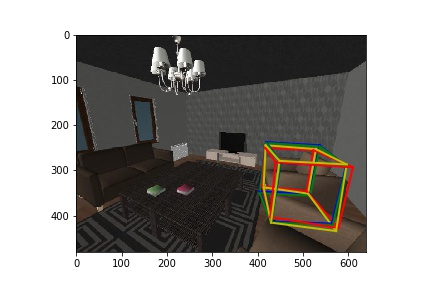
\includegraphics[width=\linewidth]{results/suncg/000007_color.jpg}
  \end{subfigure}
  \begin{subfigure}[b]{0.32\linewidth}
    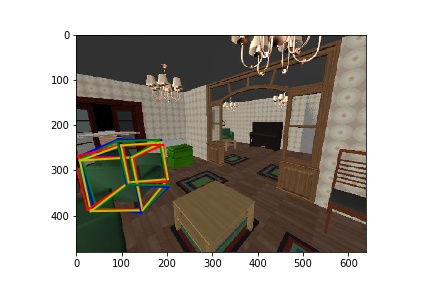
\includegraphics[width=\linewidth]{results/suncg/000017_color.jpg}
  \end{subfigure}
  \begin{subfigure}[b]{0.32\linewidth}
    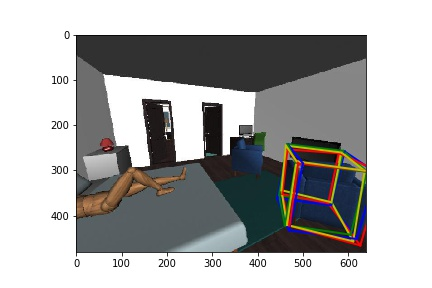
\includegraphics[width=\linewidth]{results/suncg/000020_color.jpg}
  \end{subfigure}
  \begin{subfigure}[b]{0.32\linewidth}
    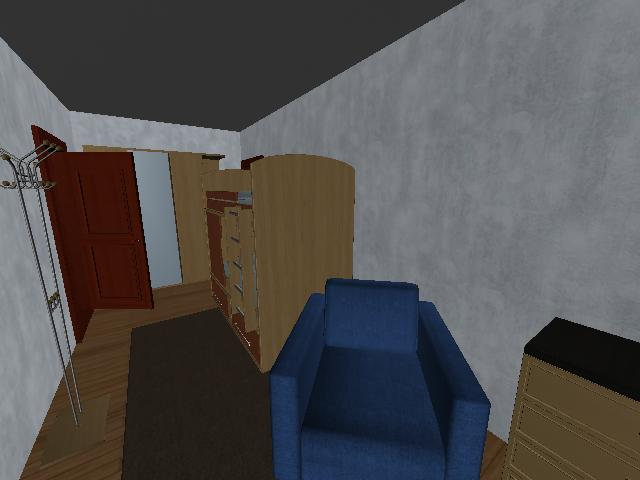
\includegraphics[width=\linewidth]{results/suncg/000031_color.jpg}
  \end{subfigure}
  \begin{subfigure}[b]{0.32\linewidth}
    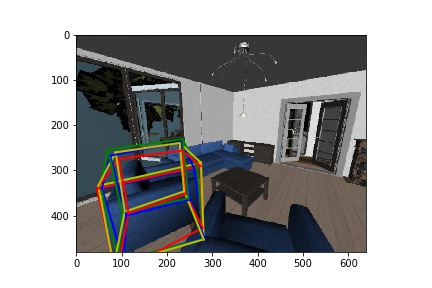
\includegraphics[width=\linewidth]{results/suncg/000034_color.jpg}
  \end{subfigure}
  \begin{subfigure}[b]{0.32\linewidth}
    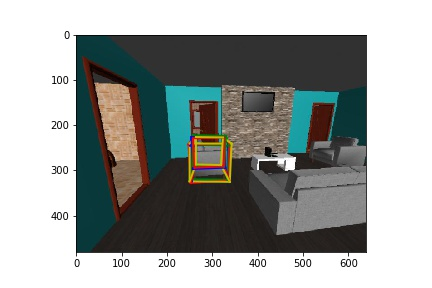
\includegraphics[width=\linewidth]{results/suncg/000045_color.jpg}
  \end{subfigure}
  \begin{subfigure}[b]{0.32\linewidth}
    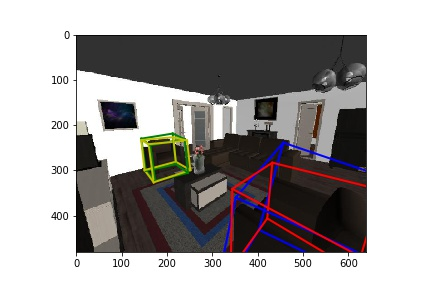
\includegraphics[width=\linewidth]{results/suncg/000050_color.jpg}
  \end{subfigure}
  \begin{subfigure}[b]{0.32\linewidth}
    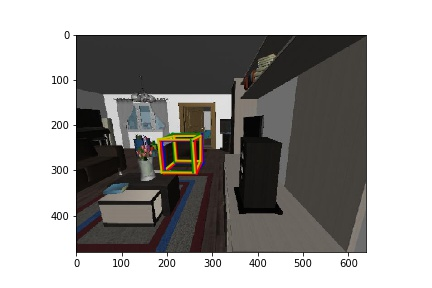
\includegraphics[width=\linewidth]{results/suncg/000055_color.jpg}
  \end{subfigure}
  \begin{subfigure}[b]{0.32\linewidth}
    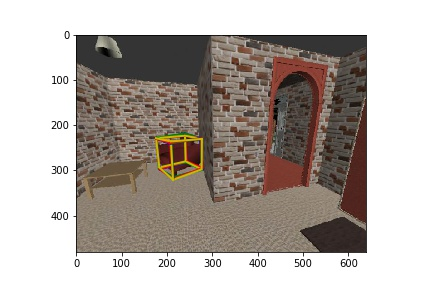
\includegraphics[width=\linewidth]{results/suncg/000057_color.jpg}
  \end{subfigure}
  \begin{subfigure}[b]{0.32\linewidth}
    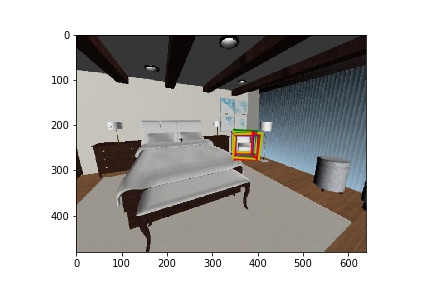
\includegraphics[width=\linewidth]{results/suncg/000058_color.jpg}
  \end{subfigure}
  \begin{subfigure}[b]{0.32\linewidth}
    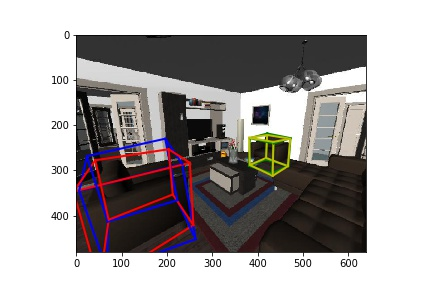
\includegraphics[width=\linewidth]{results/suncg/000060_color.jpg}
  \end{subfigure}
  \begin{subfigure}[b]{0.32\linewidth}
    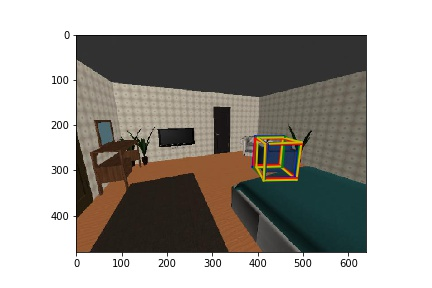
\includegraphics[width=\linewidth]{results/suncg/000061_color.jpg}
  \end{subfigure}
  \begin{subfigure}[b]{0.32\linewidth}
    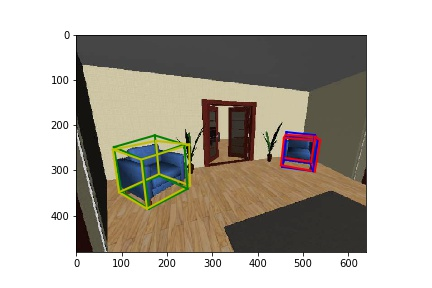
\includegraphics[width=\linewidth]{results/suncg/000066_color.jpg}
  \end{subfigure}
  \begin{subfigure}[b]{0.32\linewidth}
    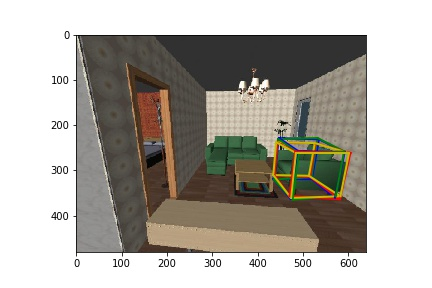
\includegraphics[width=\linewidth]{results/suncg/000073_color.jpg}
  \end{subfigure}
  \begin{subfigure}[b]{0.32\linewidth}
    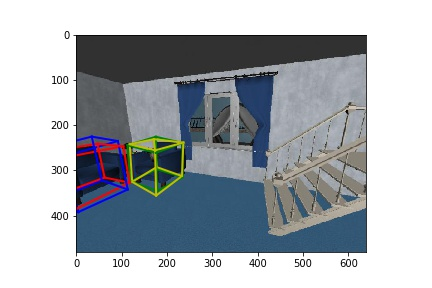
\includegraphics[width=\linewidth]{results/suncg/000096_color.jpg}
  \end{subfigure}
  \caption{Examples of results for sofa objects in SunCG test dataset}
  \label{fig:suncg}
\end{figure}

\section{Real Data}

For real data, we still have a lot of space for improvement. We will explain in more details in next chapter. However, we already achieve some good results on real data for single object camera pose detection. We get our training and testing data from 264 different scenes and in total 565 scans. Here are some results on Scannet Dataset.

Our model performs very well on training data or data from the same scene. When test on new scenes, which the network has never seen in the training period, we also get some quite good predictions. Figure \ref{fig:result_couch} shows some examples of the good results we get on couch object in ScanNet test scenes. The red bounding boxes are the ground truth and the yellow bounding  boxes are the predicted 2D points locations. As we can see, our model is robust to occlusion and different sizes of the object. Sometimes our ground truth label is not accurate due to the reasons we have explained in last chapter, and the predictions can even fix the noise and make a better bounding box than our labels. For example our ground truth label may not be upright due to noises in camera pose or incomplete construction of the object model, and the predicted bounding box can be upright and fit the object better.

\begin{figure}[h!]
  \centering
  \begin{subfigure}[b]{0.32\linewidth}
    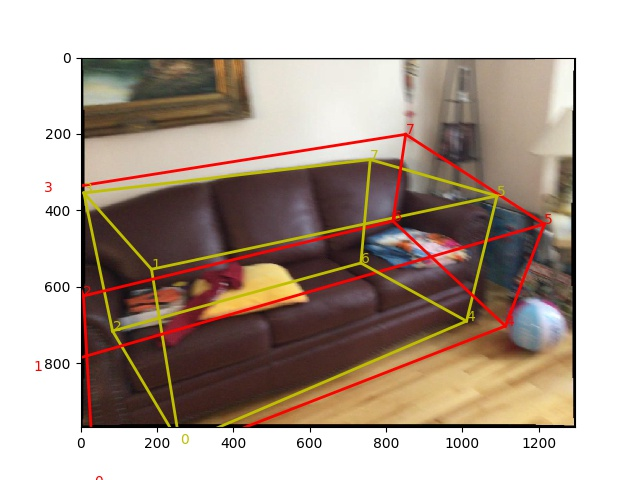
\includegraphics[width=\linewidth]{results/couch/scene0024_02_2776.jpg}
  \end{subfigure}
  \begin{subfigure}[b]{0.32\linewidth}
    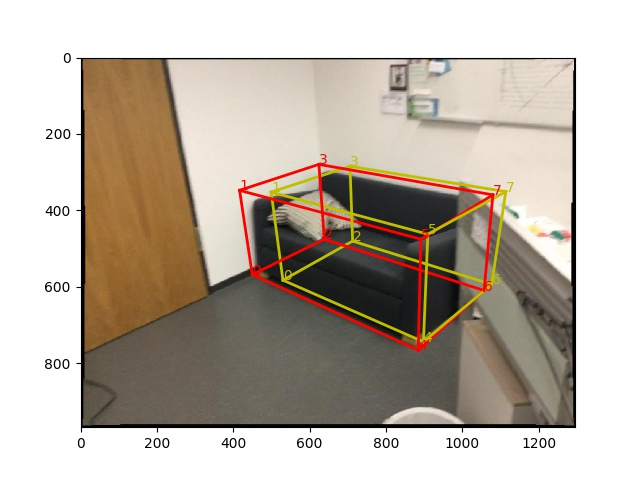
\includegraphics[width=\linewidth]{results/couch/scene0025_00_516.jpg}
  \end{subfigure}
  \begin{subfigure}[b]{0.32\linewidth}
    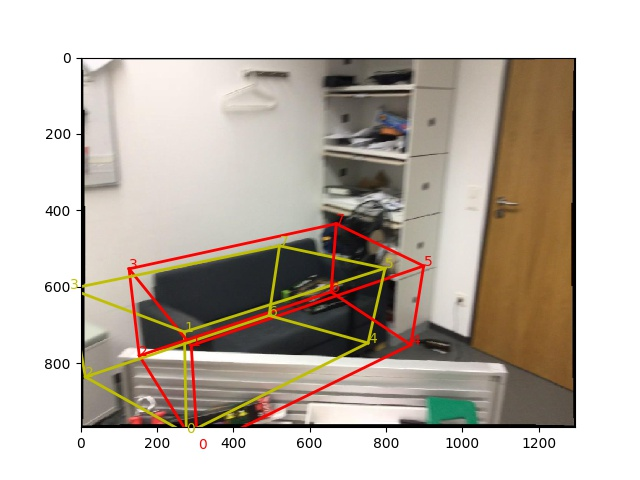
\includegraphics[width=\linewidth]{results/couch/scene0025_01_516.jpg}
  \end{subfigure}
  \begin{subfigure}[b]{0.32\linewidth}
    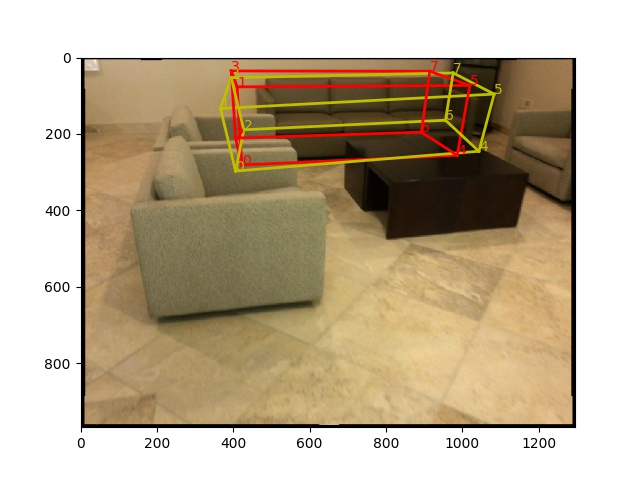
\includegraphics[width=\linewidth]{results/couch/scene0199_00_762.jpg}
  \end{subfigure}
  \begin{subfigure}[b]{0.32\linewidth}
    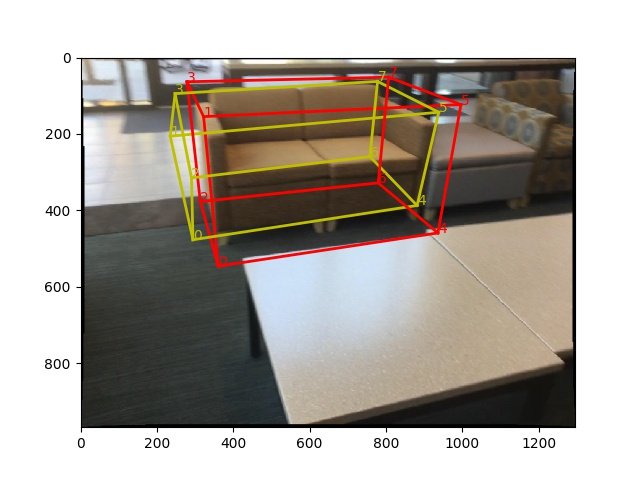
\includegraphics[width=\linewidth]{results/couch/scene0031_00_877.jpg}
  \end{subfigure}
  \begin{subfigure}[b]{0.32\linewidth}
    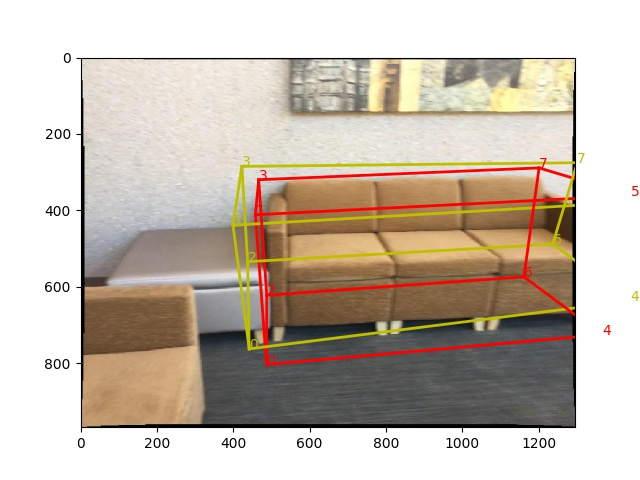
\includegraphics[width=\linewidth]{results/couch/scene0031_00_1644.jpg}
  \end{subfigure}
  \begin{subfigure}[b]{0.32\linewidth}
    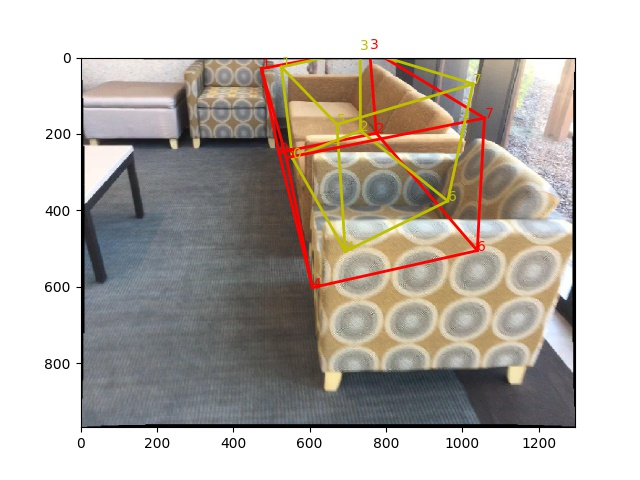
\includegraphics[width=\linewidth]{results/couch/scene0031_00_1900.jpg}
  \end{subfigure}
  \begin{subfigure}[b]{0.32\linewidth}
    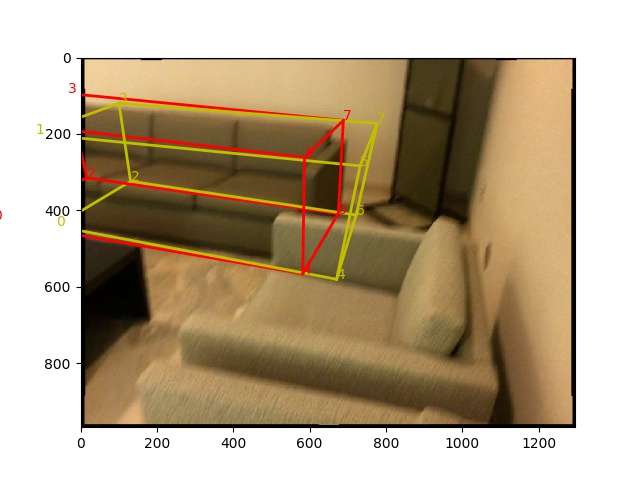
\includegraphics[width=\linewidth]{results/couch/scene0199_00_1471.jpg}
  \end{subfigure}
  \begin{subfigure}[b]{0.32\linewidth}
    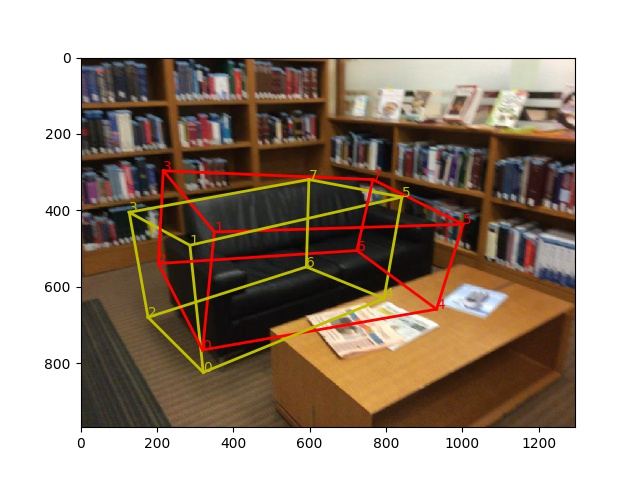
\includegraphics[width=\linewidth]{results/couch/scene0064_00_80.jpg}
  \end{subfigure}
  \begin{subfigure}[b]{0.32\linewidth}
    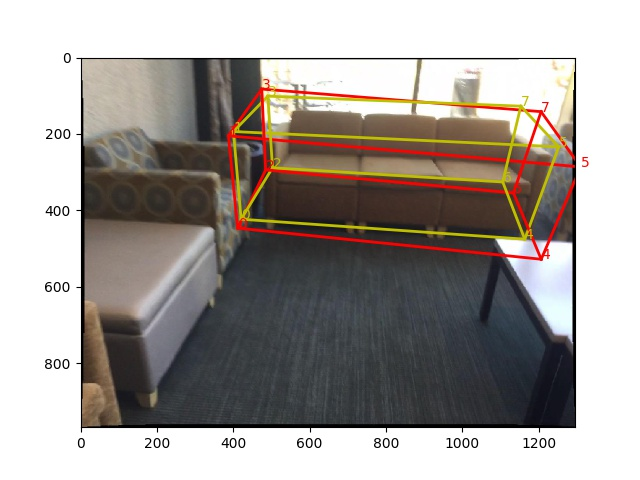
\includegraphics[width=\linewidth]{results/couch/scene0031_01_565.jpg}
  \end{subfigure}
  \begin{subfigure}[b]{0.32\linewidth}
    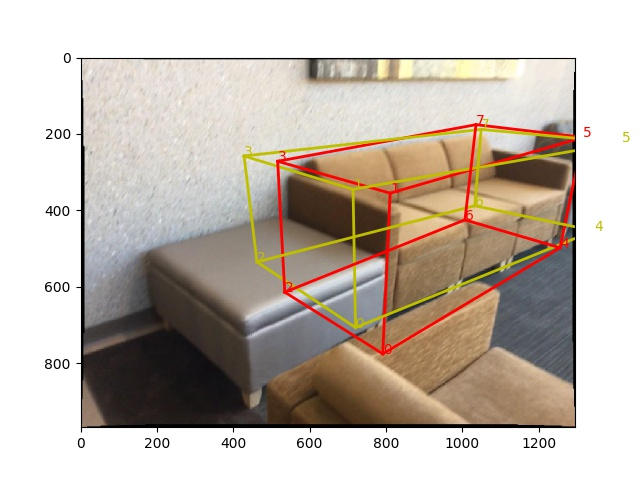
\includegraphics[width=\linewidth]{results/couch/scene0031_01_2147.jpg}
  \end{subfigure}
  \begin{subfigure}[b]{0.32\linewidth}
    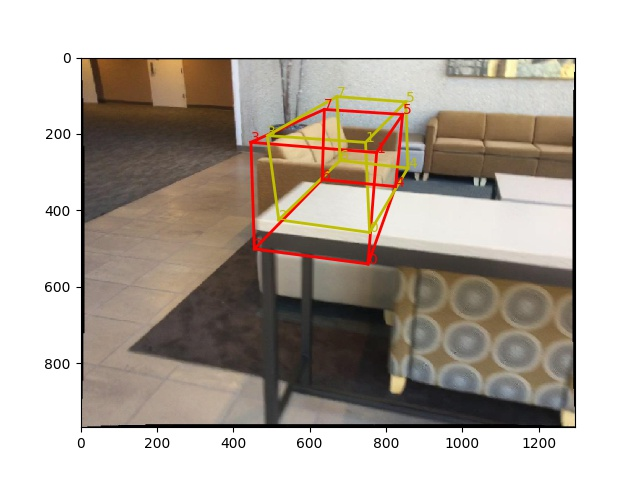
\includegraphics[width=\linewidth]{results/couch/scene0031_02_1702.jpg}
  \end{subfigure}
  \begin{subfigure}[b]{0.32\linewidth}
    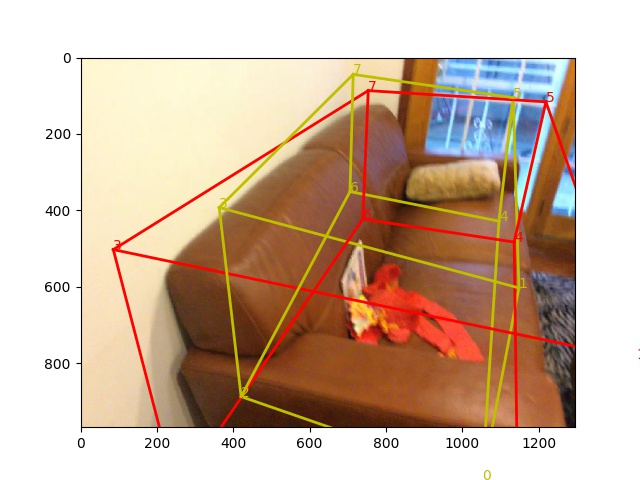
\includegraphics[width=\linewidth]{results/couch/scene0050_02_4364.jpg}
  \end{subfigure}
  \begin{subfigure}[b]{0.32\linewidth}
    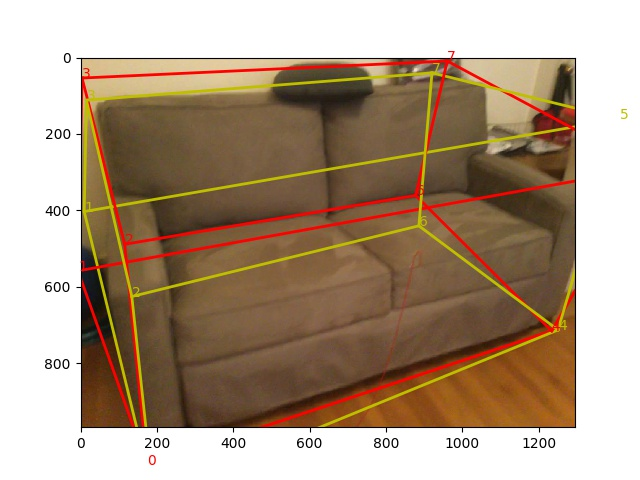
\includegraphics[width=\linewidth]{results/couch/scene0054_00_1691.jpg}
  \end{subfigure}
  \begin{subfigure}[b]{0.32\linewidth}
    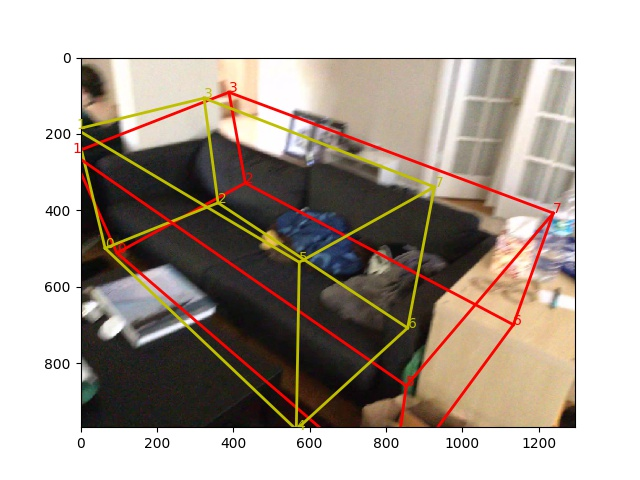
\includegraphics[width=\linewidth]{results/couch/scene0203_02_319.jpg}
  \end{subfigure}
  \caption{Examples of some good results for couch objects in ScanNet test scenes}
  \label{fig:result_couch}
\end{figure}

Figure \ref{fig:result_couch_gt_err} shows some examples on different predictions with the ground truth, but they are not wrong. In this experiment, we try to filter out those images containing multiple same category objects. However, there are some noises maintain due to incomplete construction or objects in different sizes. As we mentioned before, we filter out those non-similar object model according to the difference of the size of its bounding box with our chosen 3D model. And when we choose images containing single target category object, we check that weather there are any other objects in the same category after filtering out similar objects. This means there may still be some other objects in the same category maintain in the image but with a different size i.e. out of the range of the threshold we set for bounding box size difference. Thus, when we test on these images, there may be other object predicted instead of the labeled one. As we can see, these predictions are not false, and should not contribute to our error measurements. Some of them predicts the other object in the image in the same category. Some of them try to fit in with a quite different shape which they have never seen during training period. And some of them may detected another category object but the appearance is very similar to our target object, which are sometimes even hard to distinguish for human beings. For example sometimes the network regards the pillow on the couch as the back of another small couch, which are quite reasonable predictions.

\begin{figure}[h!]
  \centering
  \begin{subfigure}[b]{0.32\linewidth}
    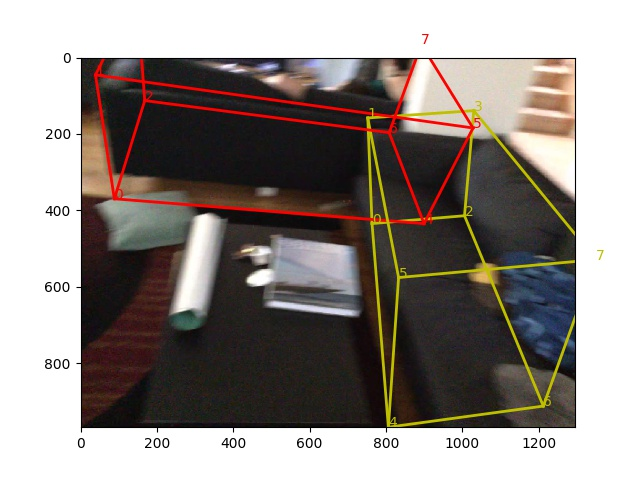
\includegraphics[width=\linewidth]{results/couch_gt_err/scene0203_02_941.jpg}
  \end{subfigure}
  \begin{subfigure}[b]{0.32\linewidth}
    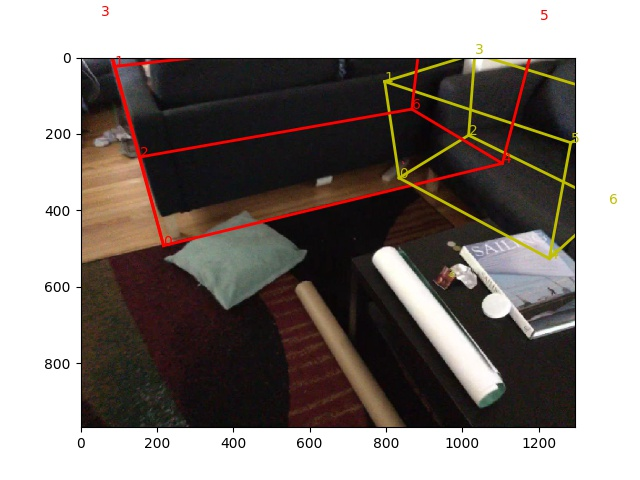
\includegraphics[width=\linewidth]{results/couch_gt_err/scene0203_01_774.jpg}
  \end{subfigure}
  \begin{subfigure}[b]{0.32\linewidth}
    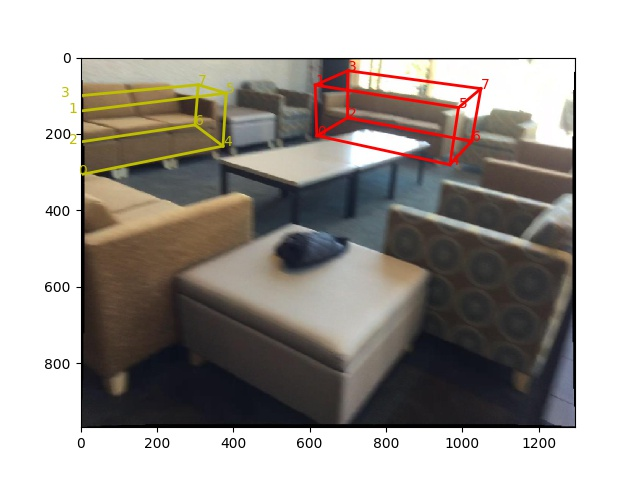
\includegraphics[width=\linewidth]{results/couch_gt_err/scene0031_00_2361.jpg}
  \end{subfigure}
  \begin{subfigure}[b]{0.32\linewidth}
    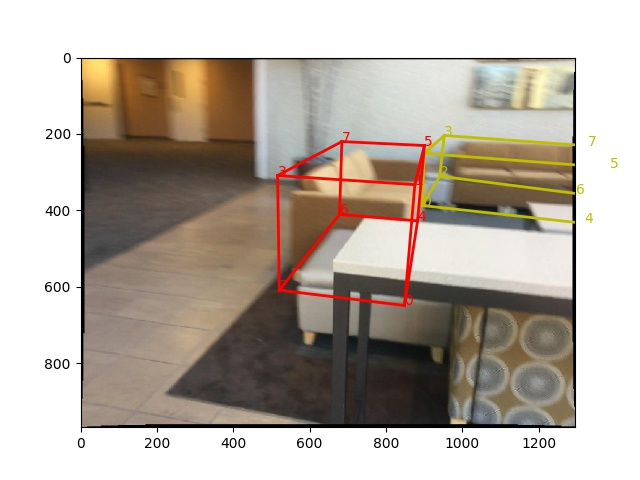
\includegraphics[width=\linewidth]{results/couch_gt_err/scene0031_01_1938.jpg}
  \end{subfigure}
  \begin{subfigure}[b]{0.32\linewidth}
    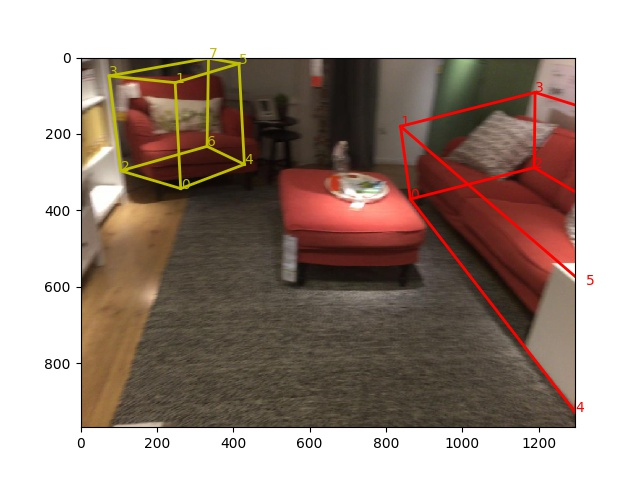
\includegraphics[width=\linewidth]{results/couch_gt_err/scene0049_00_192.jpg}
  \end{subfigure}
  \begin{subfigure}[b]{0.32\linewidth}
    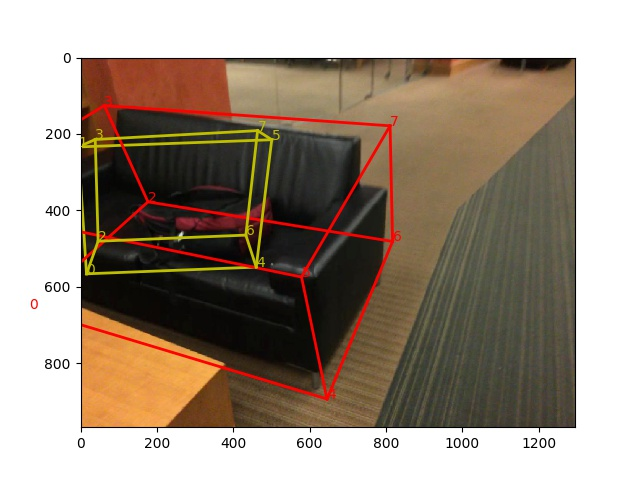
\includegraphics[width=\linewidth]{results/couch_gt_err/scene0064_00_319.jpg}
  \end{subfigure}
  \begin{subfigure}[b]{0.32\linewidth}
    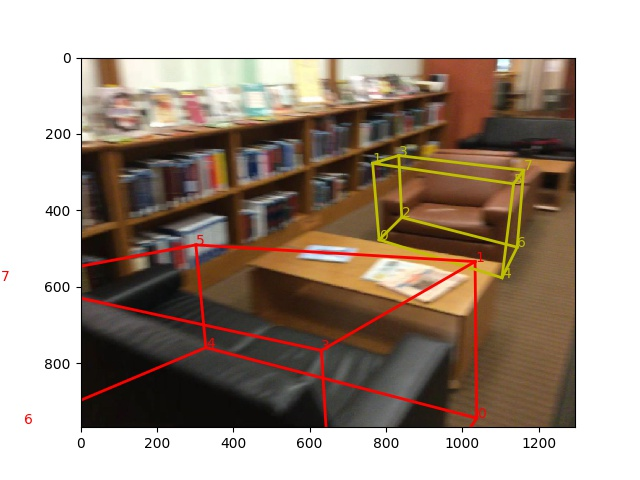
\includegraphics[width=\linewidth]{results/couch_gt_err/scene0064_00_1022.jpg}
  \end{subfigure}
  \begin{subfigure}[b]{0.32\linewidth}
    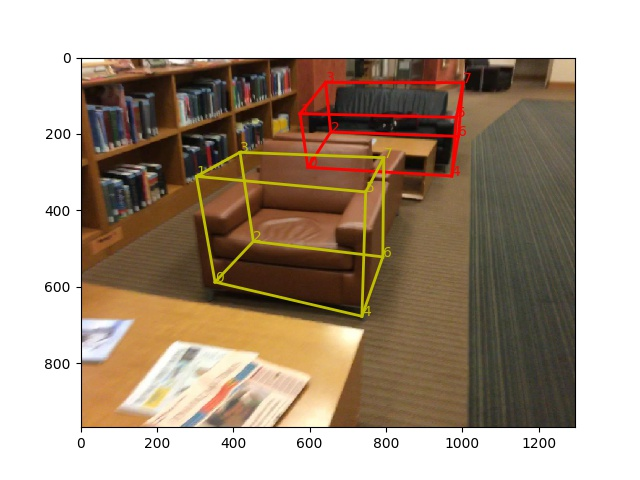
\includegraphics[width=\linewidth]{results/couch_gt_err/scene0064_00_1090.jpg}
  \end{subfigure}
  \begin{subfigure}[b]{0.32\linewidth}
    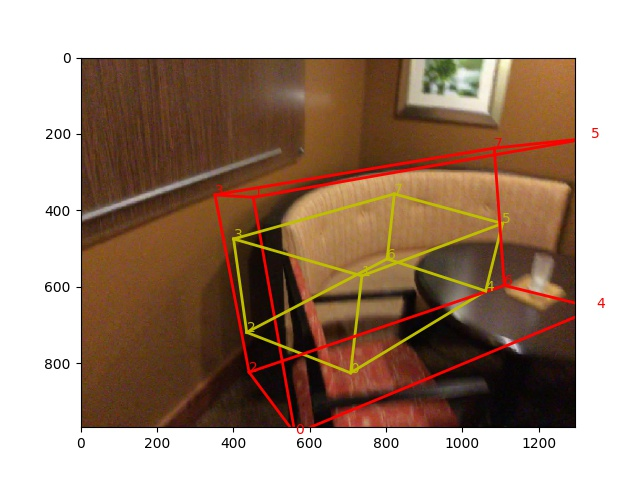
\includegraphics[width=\linewidth]{results/couch_gt_err/scene0132_00_1133.jpg}
  \end{subfigure}
  \begin{subfigure}[b]{0.32\linewidth}
    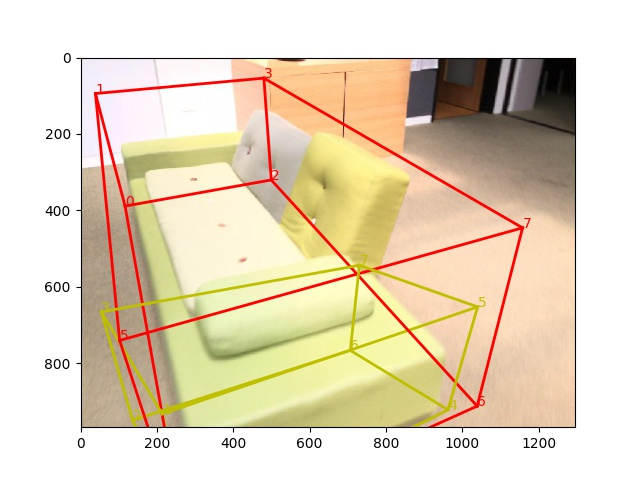
\includegraphics[width=\linewidth]{results/couch_gt_err/scene0148_00_1090.jpg}
  \end{subfigure}
  \begin{subfigure}[b]{0.32\linewidth}
    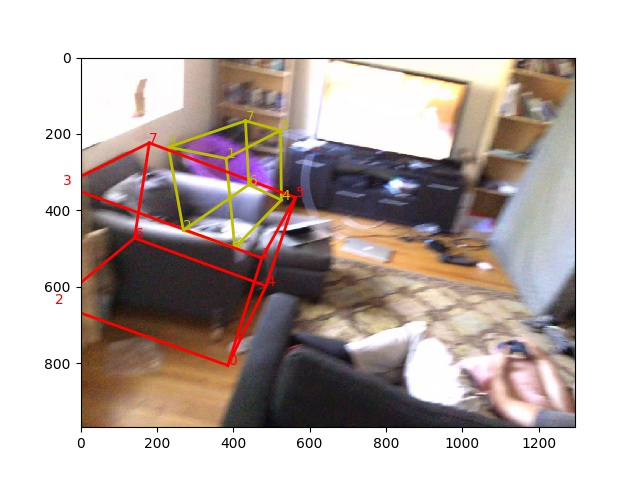
\includegraphics[width=\linewidth]{results/couch_gt_err/scene0203_02_1938.jpg}
  \end{subfigure}
  \begin{subfigure}[b]{0.32\linewidth}
    \includegraphics[width=\linewidth]{results/couch_gt_err/scene0031_02_2420.jpg}
  \end{subfigure}
  \caption{Examples of some reasonable results for couch objects in ScanNet test scenes}
  \label{fig:result_couch_gt_err}
\end{figure}

There are also a lot of failed cases. Figure \ref{fig:result_couch_err} shows these incorrect predictions. Consider the reasoning, there are less accuracy for predictions from the back of the couch. This is also reasonable for human beings, as it's a lack of important features when only the back of the couch is present in the image. The predictions are poorer for the objects having similar texture or color with the background, which is sometimes also difficult to distinguish in human eyes. The predictions are also poorer for the object containing different textures or colors itself. This may make the network partition the object and predict only part of the object. For example, the network has never seen a couch having different colors in its back, or couch with no back in some part, and the model only predict a part of the couch which contains  a back and consists of only one color/texture. And finally, those object in quite special shapes that the network has never seen during training result in poor predictions. Of course our training data size is not large enough. By enlarging the size of the training dataset, our model  may generalize better to more objects of different shapes in the same category.

\begin{figure}[h!]
  \centering
  \begin{subfigure}[b]{0.32\linewidth}
    \includegraphics[width=\linewidth]{results/couch_err/scene0234_00_368.jpg}
  \end{subfigure}
  \begin{subfigure}[b]{0.32\linewidth}
    \includegraphics[width=\linewidth]{results/couch_err/scene0031_02_1860.jpg}
  \end{subfigure}
  \begin{subfigure}[b]{0.32\linewidth}
    \includegraphics[width=\linewidth]{results/couch_err/scene0050_01_993.jpg}
  \end{subfigure}
  \begin{subfigure}[b]{0.32\linewidth}
    \includegraphics[width=\linewidth]{results/couch_err/scene0064_00_981.jpg}
  \end{subfigure}
  \begin{subfigure}[b]{0.32\linewidth}
    \includegraphics[width=\linewidth]{results/couch_err/scene0141_02_618.jpg}
  \end{subfigure}
  \begin{subfigure}[b]{0.32\linewidth}
    \includegraphics[width=\linewidth]{results/couch_err/scene0148_00_565.jpg}
  \end{subfigure}
  \begin{subfigure}[b]{0.32\linewidth}
    \includegraphics[width=\linewidth]{results/couch_err/scene0148_00_893.jpg}
  \end{subfigure}
  \begin{subfigure}[b]{0.32\linewidth}
    \includegraphics[width=\linewidth]{results/couch_err/scene0203_00_503.jpg}
  \end{subfigure}
  \begin{subfigure}[b]{0.32\linewidth}
    \includegraphics[width=\linewidth]{results/couch_err/scene0203_00_608.jpg}
  \end{subfigure}
  \begin{subfigure}[b]{0.32\linewidth}
    \includegraphics[width=\linewidth]{results/couch_err/scene0203_00_1446.jpg}
  \end{subfigure}
  \begin{subfigure}[b]{0.32\linewidth}
    \includegraphics[width=\linewidth]{results/couch_err/scene0203_02_336.jpg}
  \end{subfigure}
  \begin{subfigure}[b]{0.32\linewidth}
    \includegraphics[width=\linewidth]{results/couch_err/scene0203_02_1991.jpg}
  \end{subfigure}
  \caption{Examples of some failed results for couch objects in ScanNet test scenes}
  \label{fig:result_couch_err}
\end{figure}

\begin{figure}[h!]
  \centering
  \begin{subfigure}[b]{0.32\linewidth}
    \includegraphics[width=\linewidth]{results/table/scene0061_01_1531.jpg}
  \end{subfigure}
  \begin{subfigure}[b]{0.32\linewidth}
    \includegraphics[width=\linewidth]{results/table/scene0072_01_516.jpg}
  \end{subfigure}
  \begin{subfigure}[b]{0.32\linewidth}
    \includegraphics[width=\linewidth]{results/table/scene0125_00_45.jpg}
  \end{subfigure}
  \begin{subfigure}[b]{0.32\linewidth}
    \includegraphics[width=\linewidth]{results/table/scene0155_02_45.jpg}
  \end{subfigure}
  \begin{subfigure}[b]{0.32\linewidth}
    \includegraphics[width=\linewidth]{results/table/scene0196_00_1405.jpg}
  \end{subfigure}
  \begin{subfigure}[b]{0.32\linewidth}
    \includegraphics[width=\linewidth]{results/table/scene0244_00_319.jpg}
  \end{subfigure}
  \caption{Examples of the some good results for table objects in ScanNet test scenes}
  \label{fig:result_table}
\end{figure}

\begin{figure}[h!]
  \centering
  \begin{subfigure}[b]{0.32\linewidth}
    \includegraphics[width=\linewidth]{results/chair/scene0005_01_1152.jpg}
  \end{subfigure}
  \begin{subfigure}[b]{0.32\linewidth}
    \includegraphics[width=\linewidth]{results/chair/scene0006_00_691.jpg}
  \end{subfigure}
  \begin{subfigure}[b]{0.32\linewidth}
    \includegraphics[width=\linewidth]{results/chair/scene0006_02_2664.jpg}
  \end{subfigure}
  \begin{subfigure}[b]{0.32\linewidth}
    \includegraphics[width=\linewidth]{results/chair/scene0030_00_336.jpg}
  \end{subfigure}
  \begin{subfigure}[b]{0.32\linewidth}
    \includegraphics[width=\linewidth]{results/chair/scene0030_02_364.jpg}
  \end{subfigure}
  \begin{subfigure}[b]{0.32\linewidth}
    \includegraphics[width=\linewidth]{results/chair/scene0041_01_243.jpg}
  \end{subfigure}
  \begin{subfigure}[b]{0.32\linewidth}
    \includegraphics[width=\linewidth]{results/chair/scene0045_01_1384.jpg}
  \end{subfigure}
  \begin{subfigure}[b]{0.32\linewidth}
    \includegraphics[width=\linewidth]{results/chair/scene0056_00_1932.jpg}
  \end{subfigure}
  \begin{subfigure}[b]{0.32\linewidth}
    \includegraphics[width=\linewidth]{results/chair/scene0127_00_516.jpg}
  \end{subfigure}
  \begin{subfigure}[b]{0.32\linewidth}
    \includegraphics[width=\linewidth]{results/chair/scene0131_01_762.jpg}
  \end{subfigure}
  \begin{subfigure}[b]{0.32\linewidth}
    \includegraphics[width=\linewidth]{results/chair/scene0131_01_877.jpg}
  \end{subfigure}
  \begin{subfigure}[b]{0.32\linewidth}
    \includegraphics[width=\linewidth]{results/chair/scene0138_00_119.jpg}
  \end{subfigure}
  \begin{subfigure}[b]{0.32\linewidth}
    \includegraphics[width=\linewidth]{results/chair/scene0163_00_2083.jpg}
  \end{subfigure}
  \begin{subfigure}[b]{0.32\linewidth}
    \includegraphics[width=\linewidth]{results/chair/scene0163_01_150.jpg}
  \end{subfigure}
  \begin{subfigure}[b]{0.32\linewidth}
    \includegraphics[width=\linewidth]{results/chair/scene0181_02_516.jpg}
  \end{subfigure}
  \begin{subfigure}[b]{0.32\linewidth}
    \includegraphics[width=\linewidth]{results/chair/scene0181_03_977.jpg}
  \end{subfigure}
  \begin{subfigure}[b]{0.32\linewidth}
    \includegraphics[width=\linewidth]{results/chair/scene0204_00_9.jpg}
  \end{subfigure}
  \begin{subfigure}[b]{0.32\linewidth}
    \includegraphics[width=\linewidth]{results/chair/scene0249_00_1127.jpg}
  \end{subfigure}
  \caption{Examples of the some good results for chair objects in ScanNet test scenes}
  \label{fig:result_chair}
\end{figure}

For table objects, we do not get much good predictions. The tables in the dataset are in a huge variety of shapes and styles, which makes the learning a difficult task. A main problem of table objects is that tables are also usually rotation invariant, i.e. a rectangle table is exactly the same after rotating 180 degrees in xy plane, and a square table is rotation invariant for every 90 degrees. A round table may even be rotation invariant in any angle of rotation in xy plane. However, our loss function calculates loss for every corresponding points between prediction and ground truth and didn't deal with this rotation variant case. Thus, there is a problem on our loss function, and we will discuss this further in next chapter.

We also have some good results for chairs. Some examples of good results are shown in Figure \ref{fig:result_chair}. The main constraint is that in most of the cases chairs are occluded by the table over it or are occupied by lots of things on it. These reasons pull down the accuracy.
\chapter{Limitations and Future Work}

Dummy text.

\section{SIXD}
\label{sec:SIXD}
Although SIXD tollkit can help us generate quite a lot different views of the object in random textures, the views we generated are still not realistic enough.

To adress these limitations, one of the future work we can do is to adjust the initial orientation of the 3D object model so that most of the camera views have a fixed upright direction aligned to z=1. Also, automatically filtering out some unrealistic views such as the view from the bottom of the object is also necessary. Since in real indoor environment, we rarely see the furniture from a view to the bottom of it. The random background utilized should better be of indoor environments containing recognizable furnitures. And if possible, it would be great if the floor can be detected and put the object onto floor level so that it is not obviously floating in the air.

\section{SunCG}
random texture, random x scale
other objects

predict multiple classes

\subsection{Example Subsection}

Dummy text.

\subsubsection{Example Subsubsection}

Dummy text.

\paragraph{Example Paragraph}

Dummy text.

\subparagraph{Example Subparagraph}

Dummy text.


3D model similar to our specified model

 intrinsic parameter


%\appendix

%\chapter{Dummy Appendix}

You can defer lengthy calculations that would otherwise only interrupt
the flow of your thesis to an appendix.


\backmatter

\bibliographystyle{plain}
\bibliography{refs}

\includepdf[pages={-}]{declaration-originality.pdf}

\end{document}
